\section{Interpolation durch Polynome}

$\Pi_n$ bezeichne den Vektorraum der Polynome von Höchstgrad $n$ mit der üblichen Addition und Skalarmultiplikation. Für jedes $p\in\Pi_n$ gibt es $a_0,\dots,a_n\in\real$, sodass
\begin{align}
	\label{1.2}
	p(x) = a_nx^n+a_{n-1}x^{n-1}+\dots+a_1x+a_0
\end{align}
und umgekehrt.

\subsection{Existenz und Eindeutigkeit}

\begin{proposition}
	Zu $n+1$ Datenpaaren $(x_0,f_0),\dots,(x_n,f_n)$ mit paarweise verschiedenen Stützstellen existiert genau ein Polynom $p\in\Pi_n$, dass die Interpolationsbedingung  \cref{interpolationsbedingung} erfüllt.
\end{proposition}
\begin{proof}
	\begin{itemize}
		\item Existenz: Sei $j\in\{0,\dots,n\}$ und $L_j:\real\to\real$ mit
		\begin{align}
			L_j(x) := \prod_{\substack{i=0\\ i\neq j}}^{n} \frac{x-x_i}{x_j-x_i}= \frac{(x-x_0)\cdot\dots\cdot(x-x_{j-1})(x-x_{j+1})\cdot\dots\cdot(x-x_n)} {(x_j-x_0)\cdot\dots\cdot(x_j-x_{j-1})(x_j-x_{j+1})\cdot\dots\cdot(x_j-x_n)}\notag
		\end{align}
		das \begriff[Basispolynom!]{\person{Lagrange}-Basispolynom} vom Grad $n$. Offenbar gilt $L_j\in\Pi_n$ und 
		\begin{align}
			\label{1.3}
			L_j(x_k)=\begin{cases}
				1 & k=j \\ 0 & k\neq j
			\end{cases} = \delta_{jk}
		\end{align}
		Definiert man $p:\real\to\real$ durch
		\begin{align}
			\label{1.4}
			p(x) := \sum_{j=0}^{n} f_j\cdot L_j(x)
		\end{align}
		so ist $p\in\Pi_n$ und außerdem erfüllt $p$ wegen \cref{1.3} die Interpolationsbedingung \cref{interpolationsbedingung}
		\item Eindeutigkeit: Angenommen es gibt Interpolierende $p,\tilde{p}\in\Pi_n$ mit $p\neq\tilde{p}$. Dann folgt $p-\tilde{p}\in\Pi_n$ und $(p-\tilde{p})(x_k)=p(x_k)-\tilde{p}(x_k)=0$ für $k=0,\dots,n$. Also hat $(p-\tilde{p})$ mindestens $n+1$ Nullstellen, hat aber Grad $n$. Das heißt, dass $(p-\tilde{p})$ das Nullpolynom sein muss.
	\end{itemize}
\end{proof}

\begin{*definition}[Interpolationspolynom]
	Das Polynom, dass die Interpolationsbedingung erfüllt, heißt \begriff{Interpolationspolynom} zu $(x_0,f_0),\dots,(x_n,f_n)$.
\end{*definition}

\begin{remark}
	\begin{itemize}
		\item Die Darstellung \cref{1.4} heißt \begriff{\person{Lagrange}-Form} des Interpolationspolynoms.
		\item Um mittels \cref{1.4} einen Funktionswert $p(x)$ zu berechnen, werden $\mathcal{O}(n^2)$ Operationen genötigt; bei gleichabständigen Stützstellen kann man diesen Aufwand auf $\mathcal{O}(n)$ verringern. Ändern sich die Stützwerte, kann man durch Wiederverwendung von den $L_j(x)$ das $p(x)$ in $\mathcal{O}(n)$ Operationen berechnen.
		\item Man kann zeigen, dass $L_0$ bis $L_n$ eine Basis von $\Pi_n$ bilden.
	\end{itemize}
\end{remark}

\subsection{\person{Newton}-Form des Interpolationspolynoms}

\begin{align}
	\label{1.5}
	p(x) = c_0 + c_1(x-x_0)+c_2(x-x_0)(x-x_1)+\dots+c_n(x-x_0)\dots(x-x_{n-1})
\end{align}
mit Koeffizienten $c_0,\dots,c_n\in\real$. Die Berechnung des Koeffizienten $c_j$ kann rekursiv durch Ausnutzen der Interpolationsbedingung \cref{interpolationsbedingung} erfolgen. Für $c_0$ erhält man
\begin{align}
	f_0 \overset{!}{=} p(x_0) = c_0 \notag
\end{align}
Seien $c_0$ bis $c_{j-1}$ bereits ermittelt. Dann folgt:
\begin{align}
	f_j \overset{!}{=} p(x_j) = \underbrace{c_0 + \sum_{k=1}^{j-1} c_k(x_j-x_0)\dots(x_j-x_{k-1})}_{\text{bekannt}} + c_j \underbrace{(x_j-x_0)\dots(x_j-x_{j-1})}_{\text{bekannt}}\notag
\end{align} 

\begin{remark}
	\begin{itemize}
		\item Der Aufwand um die Koeffizienten $c_0,\dots,c_n$ zu ermitteln ist $\mathcal{O}(n^2)$. Kommt ein Datenpaar hinzu, kann man \cref{1.5} um einen Summanden erweitern und mit $\mathcal{O}(n)$ Operationen $c_{n+1}$ bestimmen.
		\item Sind die Koeffizienten $c_0,\dots,c_n$ in \cref{1.5} bekannt, dann benötigt man zur Berechnung von $p(x)$ $\mathcal{O}(n)$ Operationen.
		\item Die Polynome $N_0,\dots,N_n:\real\to\real$ mit 
		\begin{align}
			N_0 = 1\quad\text{und}\quad N_j=(x-x_0)\dots(x-x_{j-1})\notag
		\end{align}
	heißen \begriff[Basispolynom!]{\person{Newton}-Basispolynome} und bilden eine Basis von $\Pi_n$.
	\end{itemize}
\end{remark}

Die Koeffizienten $c_0,\dots,c_n$ ergeben sich wegen \cref{1.2} auch als Lösung des folgenden linearen Gleichungssystems:
\begin{align}
	\begin{pmatrix}
		1 & & & & \\
		1 & (x_1-x_0) & & & \\
		1 & (x_2-x_0) & (x_2-x_0)(x_2-x_1) & & \\
		\vdots & \vdots & \vdots & \ddots & \\
		1 & (x_n-x_0) & (x_n-x_0)(x_n-x_1) & \dots & \prod\limits_{i=0}^{n-1} (x_n-x_i)
	\end{pmatrix}\cdot
	\begin{pmatrix}
		c_0 \\ c_1 \\ c_2 \\ \vdots \\ c_n
	\end{pmatrix} = 
	\begin{pmatrix}
	f_0 \\ f_1 \\ f_2 \\ \vdots \\ f_n
	\end{pmatrix}\notag
\end{align}
Die Systemmatrix dieses linearen Gleichungssystems ist eine reguläre untere Dreiecksmatrix.

Zu effizienten Berechnung eines Funktionswertes $p(x)$ nach \cref{1.5} mit gegebenen Koeffizienten $c_0,\dots,c_n$ kann man das \begriff{\person{Horner}-Schema} anwenden. Überlegung für $n=3$.
\begin{align}
	p(x) &= c_0 + c_1(x-x_0) + c_2(x-x_0)(x-x_1) + c_3(x-x_0)(x-x_1)(x-x_2) \notag \\
	&= c_0 + (x-x_0)\Big[ c_1 + (x-x_1)\left[ c_2 + (x-x_2)c_3\right]\Big]\notag
\end{align}
Für beliebiges $n$ liefert das den folgenden Algorithmus:

\begin{algorithm}[\person{Horner}-Schema für \person{Newton}-Form]
	Input: $n$, $x$, $c_0$,..., $c_n$, $x_0$,..., $x_n$
\begin{lstlisting}
p = %$c_n$%
do j = n-1, 0, -1
 p = %$c_j$% + (x - %$x_j$%)p
end do
\end{lstlisting}
\end{algorithm}

\subsection{Interpolationsfehler}

\begin{*definition}[Maximum-Norm]
	Die Norm
	\begin{align}
		\Vert g\Vert_\infty := \max\limits_{x\in[a,b]}\vert g(x)\vert\quad\text{für } g\in C[a,b]\notag
	\end{align}
	definiert die \begriff{Maximum-Norm} in $C[a,b]$.
\end{*definition}

\begin{proposition}
	Sei $f\in C[a,b]$. Dann existiert zu jedem $\varepsilon>0$ ein Polynom $p_\varepsilon$ mit $\Vert f-p_\varepsilon\Vert\le\varepsilon$.
\end{proposition}

Also liegt die Menge aller Polynome (beliebig hohen Grades) direkt in $C[a,b]$.

\begin{definition}[Stützstellensystem]
	\begriff{Stützstellensystem}: $a\le x_0^{(n)} < ... < x_n^{(n)} \le b$. Weiterhin bezeichne $p_n\in\Pi_n$ das zu den Datenpaaren $(x_k^{(n)},f(x_k^{(n)}))$ gehörende eindeutig bestimmte Interpolationspolynom.
\end{definition}

\begin{proposition}[Satz von \person{Faber} 1914]
	Zu jedem Stützstellensystem gibt es $f\in C[a,b]$, sodass $(p_n)$ nicht gleichmäßig gegen $f$ konvergiert. \\
	$\Vert p_n-f\Vert_\infty\to 0$ bedeutet, dass $(p_n)$ gleichmäßig gegen $f$ konvergiert.
\end{proposition}

Nach einem Resultat von \person{Erdös}/\person{Vertesi} (1980) gilt sogar, dass $(p_n(x))$ fast überall divergiert.

\begin{example}[\person{Runge}]
	$f:\real\to\real$, $f(x)=\frac{1}{1+25x^2}$ \\
	äquidistante Stützstellen $x_0,...,x_n$, $p\in\Pi_n$ als Interpolationspolynom
	\begin{center}
		\begin{tabular}{l|p{8cm}}
			\textbf{Stützstellen} & \textbf{interpoliertes Polynom} \\
			\hline
			2 & $1-\frac{25x^2}{26}$ \\
			\hline
			4 & $3,31565x^4 - 4,27719x^2 + 1$ \\
			\hline
			8 & $53,6893x^8 - 102,815x^6 + 61,3672x^4 - 13,203x^2 + 1$ \\
			\hline
			16 & $15403,1x^{16} - 49713,5x^{14} + 63743,8x^{12} - 41870x^{10} + 15206x^8 - 3100,35x^6 + 351,984x^4 - 22,7759x^2 + 1$
		\end{tabular}
	\end{center}
	\begin{center}\begin{tikzpicture}
		\begin{axis}[
		xmin=-1, xmax=1, xlabel=$x$,
		ymin=-1.5, ymax=3, ylabel=$y$,
		samples=1200,
		axis y line=middle,
		axis x line=middle,
		width=0.9\textwidth,
		height=0.5\textheight,
		restrict x to domain=-1:1,
		restrict y to domain=-1.5:2
		]
		\addplot+[mark=none, line width=1mm] {1/(1+25*x^2)};
		\addlegendentry{Runge-Funktion}
		\addplot+[mark=none] {1-(25*x^2)/(26)};
		\addlegendentry{Interpolation 2 Stützstellen}
		\addplot+[mark=none, color=darkgreen] {3.31565*x^4 - 4.27719*x^2 + 1};
		\addlegendentry{Interpolation 4 Stützstellen}
		\addplot+[mark=none, color=black] {53.6893*x^8 - 102.815*x^6 + 61.3672*x^4 - 13.203*x^2 + 1};
		\addlegendentry{Interpolation 8 Stützstellen}
		\addplot+[mark=none, color=lime] {15403.1*x^16 - 49713.5*x^14 + 63743.8*x^12 - 41870*x^10 + 15206*x^8 - 3100.35*x^6 + 351.984*x^4 - 22.7759*x^2 + 1};
		\addlegendentry{Interpolation 16 Stützstellen}
		\end{axis}
		\end{tikzpicture}\end{center}
\end{example}

\begin{*anmerkung}
	Wer mit Mathematica selber diese Polynome berechnen will, muss folgende Befehle benutzen:
	\begin{itemize}
	\item Funktion definieren: \verb|f[x_]:=1/(1+25x^2)|
	\item Interpolationspolynome ausrechnen: \texttt{Expand[InterpolatingPolynomial[Table[\{i,f[i]\},} \\
	\texttt{\{i,-1,-1,Schrittweite\}],\{x\}]]}
	\item plotten: \texttt{Plot[{f[x],InterpolatingPolynomial[Table[\{i,f[i]\},\{i,-1,-1,Schrittweite\}} \\
	\texttt{],\{x\}]},\{x,-1,1\}]}
	\end{itemize}
\end{*anmerkung}

\begin{proposition}
	\proplbl{1_2_9}
	Sei $f\in C^{n+1}[a,b]$ und gelte $a\le x_0<...<x_n\le b$. Mit $p_n\in\Pi_n$ werde das zu den Datenpaaren $(x_0,f(x_0)),...,(x_n,f(x_n))$ gehörende Interpolationspolynom bezeichnet. Dann existiert zu jedem $x\in[a,b]$ eine Zahl $\xi\in(a,b)$, so dass
	\begin{align}
		f(x)-p_n(x) &= \frac{f^{n+1}(\xi(x))}{(n+1)!}w(x) \quad\text{für alle }x\in[a,b] \notag \\
		\text{wobei } w(x) &= (x-x_0)\cdot ...\cdot (x-x_n)\notag
	\end{align}
\end{proposition}
\begin{proof}
	Für $x=x_k$ mit $k=0,...,n$ ist nicht zu zeigen, da $p_n$ die Interpolationsbedingung erfüllt. Sei nun $x\in[a,b]$ fest gewählt mit $x\notin\{x_0,...,x_n\}$. Weiter seien
	\begin{align}
		K=\frac{f(x)-p_n(x)}{w(x)} \quad\text{und }\quad F:\begin{cases}
		[a,b]\to \real \\ t\mapsto f(t)-p_n(t)-Kw(t)
		\end{cases}\notag
	\end{align} 
	Man stellt unter Beachtung der Interpolationsbedingung fest, dass $F(x_0)=F(x_1)=...=F(x_n)=0$ und $F(x)=0$. Also besitzt $F$ mindestens $n+2$ paarweise verschiedene Nullstellen in $[a,b]$. Da $F\in C^{n+1}[a,b]$ erhält man durch $n+1$-fache Anwendung des Satzes von Rolle, dass $F^{(n+1)}$ mindestens eine Nullstelle $\xi(x)$ in $(a,b)$ besitzt. Also folgt 
	\begin{align}
		0=F^{(n+1)}(\xi(x))=f^{(n+1)}(\xi(x))-\underbrace{p_n^{(n+1)}(\xi(x))}_{=0} - K\underbrace{w^{(n+1)}(\xi(x))}_{\text{Konstante}}\notag
	\end{align}
	Da $w^{(n+1)}=(n+1)!$, erhält man
	\begin{align}
		K=\frac{f^{(n+1)}(\xi(x))}{(n+1)!}\notag
	\end{align}
	Da $x\in[a,b]$ beliebig gewählt war, ist die Behauptung bewiesen.
\end{proof}

\begin{example}
	Sei $f\in C^2[a,b]$ mit $\Vert f\Vert_\infty\le M$. Weiter sei $a=x_0<x_1=x_0+h=b$. Mit \propref{1_2_9} folgt:
	\begin{align}
		\vert f(x)-p_2(x)\vert &= \left|\frac{f''(\xi(x))}{2}(x-x_0)(x-x_1)\right| \notag \\
		&\le \frac{1}{2} M\cdot \lambda(x)h\cdot (1-\lambda(x))h \notag \\
		&\le \frac{1}{2} M\cdot h^2\underbrace{\lambda(x)(1-\lambda(x))}_{\le \sfrac{1}{4}} \notag \\
		&\le \frac{1}{8} M\cdot h^2\notag
	\end{align}
	\begin{center}
		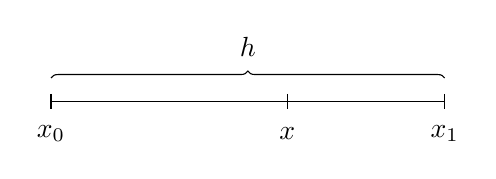
\begin{tikzpicture}
			\draw (0,0) -- (5,0);
			
			\draw (0,0.1) -- (0,-0.1);
			\draw (5,0.1) -- (5,-0.1);
			\draw (3,0.1) -- (3,-0.1);
			\node at (0,-0.4) (1) {$x_0$};
			\node at (3,-0.4) (2) {$x$};
			\node at (5,-0.4) (3) {$x_1$};
			
			\draw[decoration={brace}, decorate] (0,0.3) -- (5,0.3);
			\node at (2.5,0.7) (h) {$h$};
		\end{tikzpicture}
	\end{center}
$\Rightarrow x=x_0+\lambda\cdot(x_1-x_0)=\lambda x_1+(1-\lambda)x_0$
\end{example}